\section{Model definition}
\label{model-definition}
This Section presents how the networks used on the training set are 
structured, the second Subsection gives an overview of the performances 
on the different training sets, lastly, the Hyperparameter tuning phase
is described.

\subsection{Neural network structure}
The starting point for the neural network structure was a 
reasonable network in terms of hidden neurons to prevent over-fitting, 
indeed a high number of units in the hidden layers would end up in learning 
too much from the dataset.

The rule of thumb followed to decide hidden neurons quantity is the 
following: 
$$\#\mathit{hidden\; neurons} = \frac{2}{3}\#\mathit{input\;neurons}
+ \#\mathit{output\;neurons}$$
The next step was to decide the hidden layer number. To respect the 
number of hidden neurons, two hidden layers were considered. 
A more complex structure in terms of layers number would mean 
having a real small number of neurons per layer.

To give reference, this is the model used on the PCA training set, mentioned at 
the end of Subsection \vref{extended-dataset}, with 
120 input features.

\begin{center}
    
    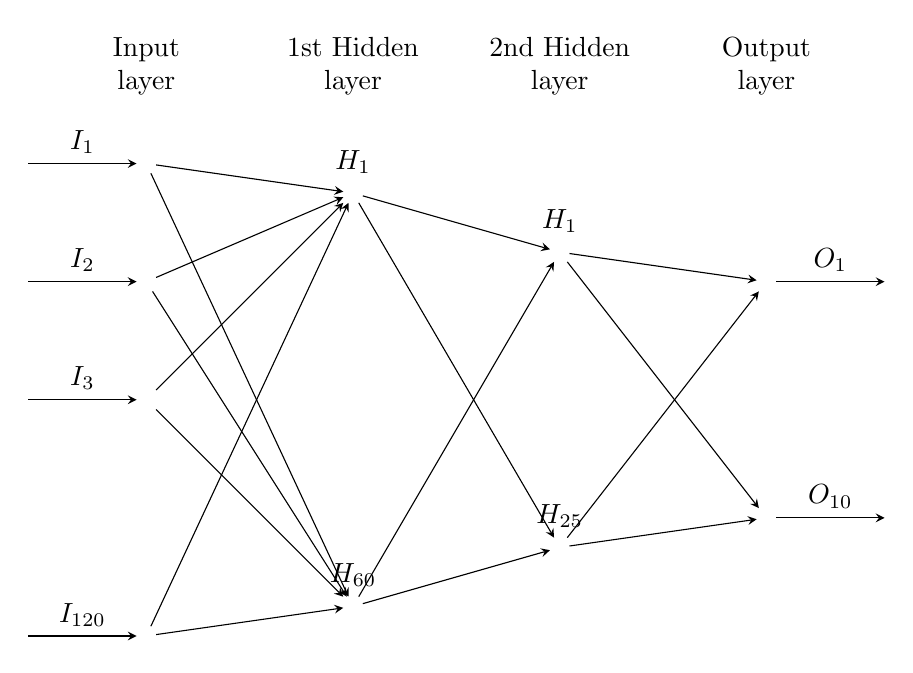
\begin{tikzpicture}[x=1.5cm, y=1.5cm, >=stealth]
        
        % layers
        \foreach \m/\l [count=\y] in {1,2,3,missing,4}
        \node [every neuron/.try, neuron \m/.try] (input-\m) at (0,2.5-\y) {};
        
        \foreach \m [count=\y] in {1,missing,2}
        \node [every neuron/.try, neuron \m/.try ] (hidden-\m) at (1.75,3-\y*1.75) {};
        
        \foreach \m [count=\y] in {1,missing,2}
        \node [every neuron/.try, neuron \m/.try ] (hidden2-\m) at (3.5,2-\y*1.25) {};
        
        \foreach \m [count=\y] in {1,missing,2}
        \node [every neuron/.try, neuron \m/.try ] (output-\m) at (5.25,1.5-\y) {};
        
        %   label
        \foreach \l [count=\i] in {1,2,3,{120}}
        \draw [<-] (input-\i) -- ++(-1,0)
        node [above, midway] {$I_{\l}$};
        
        \foreach \l [count=\i] in {1,60}
        \node [above] at (hidden-\i.north) {$H_{\l}$};
        
        \foreach \l [count=\i] in {1,25}
        \node [above] at (hidden2-\i.north) {$H_{\l}$};
        
        \foreach \l [count=\i] in {1,10}
        \draw [->] (output-\i) -- ++(1,0)
        node [above, midway] {$O_{\l}$};
        
        \foreach \i in {1,...,4}
        \foreach \j in {1,...,2}
        \draw [->] (input-\i) -- (hidden-\j);
        
        \foreach \i in {1,...,2}
        \foreach \j in {1,...,2}
        \draw [->] (hidden-\i) -- (hidden2-\j);
        
        \foreach \i in {1,...,2}
        \foreach \j in {1,...,2}
        \draw [->] (hidden2-\i) -- (output-\j);
        
        \foreach \l [count=\x from 0] in {Input, 1st Hidden, 2nd Hidden, Output}
        \node [align=center, above] at (\x*1.75,2) {\l \\ layer};
        
    \end{tikzpicture}
\end{center}

The activation function for the input and hidden layers is a \emph{Relu} 
and the output one uses a \emph{Softmax}~\cite{relu} \cite{soft}. 
The loss used is the \emph{Sparse Categorical Crossentropy loss} as it is suited 
for this kind of problems~\cite{entropy}.

As discussed in the previous Section, models with this logic for 
construction were tested on the four training sets to choose the one to tune 
the final network on.

\subsection{Initial training set results}

Section \vref{feature-extraction} talked about the four different 
training sets obtained from the dataset and, without going into details, 
stated that there was continuous improvement. This subsection presents
the results obtained on the training set. 

Note that all the random seeds used by tensorflow were fixed 
to make results reproducible.

\paragraph{Cross validation}
To estimate performance on the training set \emph{cross-validation} with 
5 folds was used~\cite{cross}. Basically the dataset is divided into five folds, 
and a model is repeatly trained on four and tested on one. 
The mean accuracy on the testing folds gives a hint about the model performance.

\paragraph{Results}
For each training set presented, a model was defined 
with the structure presented at the beginning of this Section, 
and these are the results:

\begin{center}
    \begin{tabular}{ |l|r|r| } 
        \hline
        Training set & Mean accuracy & St. deviation \\
        \hline
        132 features unscaled &  0.0669 & 0.0488 \\
        132 features scaled &  0.5201 & 0.0668 \\
        144 features scaled &  0.5586 & 0.0842 \\
        120 features reduced with PCA &  0.5608 & 0.0998 \\
        \hline
    \end{tabular}
\end{center}

There is a huge improvement after scaling the training set, after 
that small refinements were made.
As accuracy is the best on the last dataset, this was the one selected to 
perform the Hyperparameter tuning.

\subsection{Hyperparameter tuning}

Choosing the training set with PCA applied, led to the best results 
with cross validation, although the model was reasonable, it can not be the 
final one, as many parameters were left on their default value, for instance, 
\emph{learning rate} and \emph{momentum} of the optimizer were not touched. 

The main goal now is to experiments with different model parameters 
to find the best one.

\paragraph{Grid vs Random search}
Two of the most commonly used strategies in Hyperparameter optimization
are \emph{Grid} and \emph{Random Search}~\cite{random-grid}. 

In both cases we define ranges of parameters to test different combinations, 
for instance, fixed the number of neurons, one could try to find the best 
combination of learning rate and momentum that optimize accuracy on the training set.

While similar, the two methodologies differs in the amount of exploration they do.
The Grid search try all the possible combinations of parameters, while the 
Random approach fixes a number of iterations and picks an arbitrary combination each time. 

Obviously the first one is more computationally expensive than the second, if 
we fix a small amount of possible iterations, but in theory it finds a better result
than going the random route. 
Nonetheless the Grid Search can led to over-fitting, and in practice Random 
Search in preferred.

To get the best out of the two techniques, a first Random Search is performed 
on a larger parameter space, then, a Grid Search is used on much smaller 
ranges to optimize the previously found model.

\paragraph{Random search}
Starting from the model introduced in the previous Subsection, parameters are 
tweaked to find a better one.
The optimizer used is the \emph{Stochastic Gradient Descent}~\cite{sgd}.
The considered ranges for parameters for this run are: 
\begin{enumerate}
    \item \emph{Neurons}: first and last layers stay the same, while 
    the two hidden layers are tested with a number of neurons respectively 
    equals to: 
    $$60 + 2i\;\;\text{and}\;\;25 + 2j,\;\;\text{with}\;\; i, j \in \{-2,-1,0,1,2\}$$
    \item \emph{Learning rate}: $0.001, 0.01, 0.1, 0.5$
    \item \emph{Momentum}: $0.0, 0.01, 0.1, 1$
\end{enumerate}

An early stopper is used on the fit with 100 \emph{epochs}, \emph{batch size} 
is fixed at 
32, and cross validation with 5 folds is performed on each combination.
The total possible models are 400, but the search was performed with 100 iterations
in total.

The best model found was the following: 
\begin{itemize}
    \item \emph{Neurons}: 120 for input, 62 for the first hidden layer, 27 for the second, and 10 for output 
    \item \emph{Momentum}: 0.1
    \item \emph{Learning rate}: 0.1
\end{itemize}
Comparing the initial model with the one found now, a small improvement 
can be seen both in accuracy and standard deviation:
\begin{center}
    \begin{tabular}{ |l|r|r| } 
        \hline
        Model & Mean accuracy & St. deviation \\
        \hline
        Initial model & 0.5608& 0.0998\\
        Random search result & 0.5857 & 0.0715 \\
        \hline
    \end{tabular}
\end{center}

\paragraph{Grid search}
The best model from the random search was then fine-tuned with a Grid Search, 
where ranges are in the proximity of the parameters found by the previous search.

Parameters this time was:
\begin{enumerate}
    \item \emph{Neurons}: first and last layer stay the same, while 
    the two hidden layers are tested with a number of neurons respectively 
    equals to: 
    $$62 + i\;\;\text{and}\;\;27 + j,\;\;\text{with}\;\; i, j \in \{-1,0,1\}$$
    \item \emph{Learning rate}: $0.08, 0.1, 0.12$
    \item \emph{Momentum}: $0.08, 0.1, 0.12$
\end{enumerate}

The total possible models was 81, the best found is the following:
\begin{itemize}
    \item \emph{Neurons}: 120 for input, 62 for the first hidden layer, 28 for the second, and 10 for output 
    \item \emph{Momentum}: 0.12
    \item \emph{Learning rate}: 0.08
\end{itemize}
As before, a comparison shows that Grid Search fine tuned the model 
to have better accuracy, unfortunately standard deviation increased by a small 
quantity:
\begin{center}
    \begin{tabular}{ |l|r|r| } 
        \hline
        Model & Mean accuracy & St. deviation \\
        \hline
        Initial model & 0.5608& 0.0998\\
        Random search result & 0.5857 & 0.0715 \\
        Grid search result & 0.5877 & 0.0763 \\
        \hline
    \end{tabular}
\end{center}
\newpage